\subsection{Rotina de Calibração}
\label{subsec:rotina_calibracao}

Rotina responsável por realizar a identificação dos parâmetros do modelo dos motores direito e esquerdo do robô: constante de tempo; ganho de malha aberta; parâmetros do controlador \emph{FeedForward}; velocidade máxima de cada motor. Bem como calcular os ganhos para o controlador \emph{P} de forma a se obter uma resposta pré-definida em malha fechada.\\

A rotina de calibração consiste em três etapas que são repetidas para todas as configurações: motor direito para frente; motor direito para trás; motor esquerdo para frente e motor esquerdo para trás. Cada etapa é descrita a seguir: \\

% TO DO:
% ORGANIZAR E REPENSAR A FORMA DE EXIBIR AS ETAPAS
% FIGURAS ILUSTRANDO O COMPORTAMENTO GERAL DAS FUNÇÕES QUE ESTÃO SENDO USADAS NA INTERPOLAÇÃO
% PSEUDO CÓDIGOS TALVEZ

\textbf{ETAPA 1.} Estimar a zona morta e o ganho da planta em malha aberta. Para isso é realizado a coleta de $N$ pontos ($\omega$,$u$), o primeiro ponto é coletado para $u = \pm1$(valor máximo no sentido de giro atual) e são realizados sucessivos decréscimos neste valor até a parada do motor ($\omega = 0$). A aquisição destes pontos ocorre da maior velocidade para a menor, pois a zona morta será mais baixa neste sentido, devido à inércia do motor.\\

Ao se encerrar a coleta destes pontos ($\omega_{ss} = 0$ detectado) é realizado uma regressão linear por mínimos quadrados, tendo $u$ no eixo das ordenadas e $\omega$ no eixo das abscisas, o coeficiente angular dessa reta relaciona a velocidade angular ($\omega$) com o sinal de controle ($u$), já o coeficiente linear representa a zona morta, ou seja, o menor $\omega$ que pode iniciar o giro do motor (\emph{Dead Zone ($D$)}). A regressão linear é possível, apesar do comportamento não linear (como também explorado em \cite{dead_zone}) entre a velocidade e o sinal de controle e ilustrado na Figura \ref{fig:ilustracao_omega_x_pwm}, se analisado um sentido de rotação por vez.

\begin{equation}
    \omega_{ss}(u) = \alpha(u + D)
    % u(\omega) = a\omega + b
    \label{eq:omega_x_sinal_de_controle}
\end{equation}

Com os parâmetros dessa reta (Equação \ref{eq:omega_x_sinal_de_controle}) é possível estimar o ganho de malha aberta da planta da seguinte forma:

\begin{equation}
    K_m = \alpha(u_{max} + D)
    % K_m = \frac{(u_{max} - b)}{a}
\end{equation}

A Figura \ref{fig:ilustracao_omega_x_pwm} apresenta uma ilustração da relação entre o \emph{PWM} (sinal de controle) e a velocidade de regime $\omega_{ss}$ do motor.

\begin{figure}[H]
    \centering
    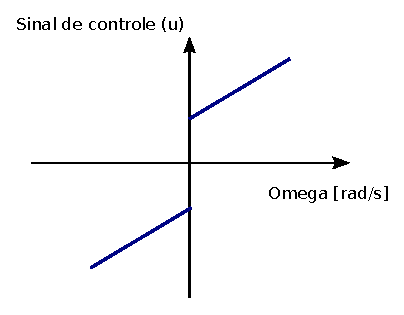
\includegraphics[width=0.5\textwidth]{figuras/ilustracoes/omega_x_sinal_controle.eps}
    \caption{Comportamento da curva $\omega_{ss}(u)$.}
    \label{fig:ilustracao_omega_x_pwm}
    \fonte{Própria.}
\end{figure}

    
\textbf{ETAPA 2.} Estimar a constante de tempo. Para obter a constante de tempo da planta na configuração atual, faz-se uso mais uma vez de interpolação por \textit{MMQ} e tira-se proveito do conhecimento do ganho da planta para simplificar e tornar possível essa interpolação de forma simples. Para estimar a constante de tempo obtém-se $M$ pontos ($t$,$\omega$) e aplica-se o \textit{MMQ} para uma interpolação linear, para isso é necessário fazer a seguinte alteração:
    

\begin{align*}
    \omega(t) &= K\left( 1 - e^{-t/T_m} \right)\\
    \ln{\omega(t)} &= \ln\left[K( 1 - e^{-t/T_m})\right]\\
    \ln\left(1 - \frac{\omega(t)}{K} \right) &= -\frac{t}{T_m}\\
    y_{aux}(t) &= -\frac{t}{T_m}
\end{align*}

Convertendo $\omega(t)$ para $y_{aux}(t)$ o coeficiente angular resultante da interpolação linear será: $coef.angular = -\frac{1}{T_m}$, dessa forma obtemos a constante de tempo.\\

\textbf{ETAPA 3.} Calcular os parâmetros do controlador \textit{Feedback}. O ganho do controlador proporcional se relaciona com o polo (inverso do negativo da constante de tempo desejada) desejado para o sistema em malha fechada, por meio da relação \ref{eq:calculo_do_Kp}. Esse cálculo só é possível devido à identificação dos parâmetros da planta resultante das etapas anteriores. O polo desejado para todas as configurações da planta é uma constante pré-definida, que para os experimentos apresentados neste trabalho foi de $-20$ (equivalente a um $\tau_m$ desejado de 0.08s).\\

\begin{equation}
    K_p = -\frac{\tau_m S_d + 1}{K_m}
    \label{eq:calculo_do_Kp}
\end{equation}

Sendo $S_d$ o polo desejado para o sistema em malha fechada, que é equivalente à $S_d = -1/\tau_{m_{d}}$.
    

Ao se passar por todas as configurações de motor/sentido a rotina seleciona a menor das velocidades máximas apresentada por alguma dessas configurações e armazena esta velocidade como sendo a velocidade máxima atingida pelos motores deste robô (na prática é armazenado 90\% desse valor, para dar uma margem de factibilidade), isso é importante, para assegurar que a referencia $\omega_{ref}$ seja factível para todas as configurações. \\

Por fim os resultados são armazenados na memória permanente do microcontrolador, sendo atualizado/sobrescritos apenas ao final da próxima chamada da rotina de calibração.